\section{Introduction}\label{sec_introduction}

%Many modern machine learning methods
%Hard parameter sharing (HPS) for multi-task learning is widely used in empirical research and goes back to the seminal work of \cite{C97}.
%Recent work has revived interests in this approach because it improves performance and reduces the cost of collecting labeled data \cite{R17}.
%It is generally applied by sharing the feature layers between all tasks while keeping an output layer for every task.
%Often, hard parameter sharing offers two critical advantages if successfully applied.
%First, it reduces model parameters since all tasks use the same feature space.
%Second, it reduces the amount of labeled data needed from each task by augmenting the entire training dataset.

%Hard parameter sharing works as an inductive transfer mechanism and a regularizer that reduces overfitting, both of which have great intuitive appeal \cite{R17}.
%For example, by restricting the shared space's size, HPS encourages information sharing among multiple tasks \cite{KD12}.
%Another source of inductive bias comes from the tasks and depends on datasets' properties such as sample sizes and task covariances \cite{WZR20}.
%However, how these dataset properties impact HPS has not been well established.
%It becomes increasingly important to understand HPS' formal generalization properties.
%Part of the challenge may be that HPS' generalization performance depends intricately on the sample size ratios and covariate shifts between tasks, and is not amenable to standard concentration results.
%Previous results based on Rademacher complexity or VC dimensions have considered cases where all tasks' sample sizes are equal to logarithmic factors of the feature dimension \cite{B00,MPR16}, and when all tasks' sample sizes increase simultaneously \cite{AZ05,M06}.
%For, the generalization error scales down as the sample sizes of all tasks increase, when applied to the multi-task setting \cite{B00,AZ05,M06,MPR16,WZR20}.

%This paper presents new techniques to study hard parameter sharing and establishes a number of new results.
%We consider regression analysis, which is arguably one of the most fundamental problems in statistics and machine learning.
%We are interested in the \textit{high-dimensional} setting, where each dataset's sample size and feature dimension grow linearly instead of logarithmically.
%This setting captures the fact that a single task's sample size is usually insufficient for accurate learning in many applications.
%For example, if a dataset's sample size is only a constant factor of dimension in linear regression, the variance is also constant (cf. Fact \ref{fact_tr}).
%The high-dimensional setting is challenging but is crucial for understanding how datasets' sample sizes impact generalization performance.


\subsection{Setup and motivating examples}\label{sec_mot}

We first define the data model.
Suppose we have two datasets (or tasks).
We refer the first dataset as the source and the second task as the target.
Let $i = 1$ or $2$.
Let $n_i$ be dataset $i$'s sample size.
Let $x_1^{(i)}, x_2^{\ss (i)}, \dots, x_{n_i}^{(i)}$ be the $n_i$ datapoints' $p$-dimensional covariates.
Let $y_1^{(i)}, y_2^{(i)}, \dots, y_{n_i}^{(i)}$ be these datapoints' labels.
We assume a linear model specified by an unknown model vector $\beta^{(i)} \in \real^p$ as follows:
\begin{align}
    y_j^{(i)} = \inner{x_j^{(i)}}{\beta^{(i)}} + \varepsilon_j^{(i)}, \text{ for any } j = 1,\dots,n_i, \label{eq_linear}
\end{align}
where $\varepsilon^{(i)}_j\in\real$ denotes a random noise variable with mean zero and variance $\sigma^2$.
Our goal is to learn an estimator to predict the target task given both datasets.

We learn a two-layer linear neural network with parameters $A \in \real^{p\times r}$, $B_1 \in \real^{r}$, and $B_2 \in \real^r$ by minimizing the following optimization objective:
\begin{align}\label{eq_hps}
    f(A, B_1, B_2) = \bignorm{X^{(1)} A B_1 - Y^{(1)}}_2^2 + \bignorm{X^{(2)} A B_2 - Y^{(2)}}_2^2.
\end{align}
The above two-layer neural network uses a shared feature space $A$ for both tasks while using a separate prediction head for each task.\footnote{Popular variants of the objective function \eqref{eq_hps} include adding a weight parameter to each summand and adding ridge regularization. We focus on the unweighted and unregularized objective for simplicity. All of the asymptotic limits we show below can be straightforwardly extended to weighted and regularized objectives.}
Such models are also known as \textit{hard parameter sharing} in the machine learning literature \cite{C97,R17}.
Suppose that $(\hat{A}, \hat{B}_1, \hat{B}_2)$ is a global minimizer of $f(\cdot)$.
We define the hard parameter sharing (HPS) estimator for the target task as $\hat{\beta}_2^{\MTL} \define \hat{B} \hat{A}_2$.
In order to evaluate the estimator, we will study the excess risk at a new (unseen) test datapoint from task two, denoted as $L(\hat{\beta}_2^{\MTL})$ (see Section \ref{sec_risk} for its precise definition).

As a motivating example of the above setup, we show an intriguing simulation where combining both datasets jointly results in different transfer effect on $L(\hat{\beta}_2^{\MTL})$, depending on the distance between $\beta^{(1)}$ and $\beta^{(2)}$.
Figure \ref{fig_motivation} shows the result for a setting where every entry of $X_1, X_2$ is generated from an isotropic Gaussian, and $\beta_1,\beta_2$ are generated such that $\norm{\beta^{(1)} - \beta^{(2)}}^2 \approx 2\mu^2$.
We observe that for $\mu = 0.25$, $L(\hat{\beta}_2^{\MTL})$ is always smaller than the excess risk of OLS.
For $\mu = 0.3$ or $0.35$, $L(\hat{\beta}_2^{\MTL})$ is smaller than the excess risk of OLS for a restricted range of $n_1$.
Such a scenario, where combining both datasets jointly improves over learning the target task individually, is also called a \textit{positive information transfer} \cite{PY09}.
On the other hand, for $\mu = 0.45$, HPS is always worse than OLS, thus providing a \textit{negative information transfer}.  
Our main contribution is to precisely analyze a number of interesting phenomena including the above that are prevalent in transfer learning, depending on geometries of the covariance matrices and model distances. 


\begin{figure*}
    \centering
    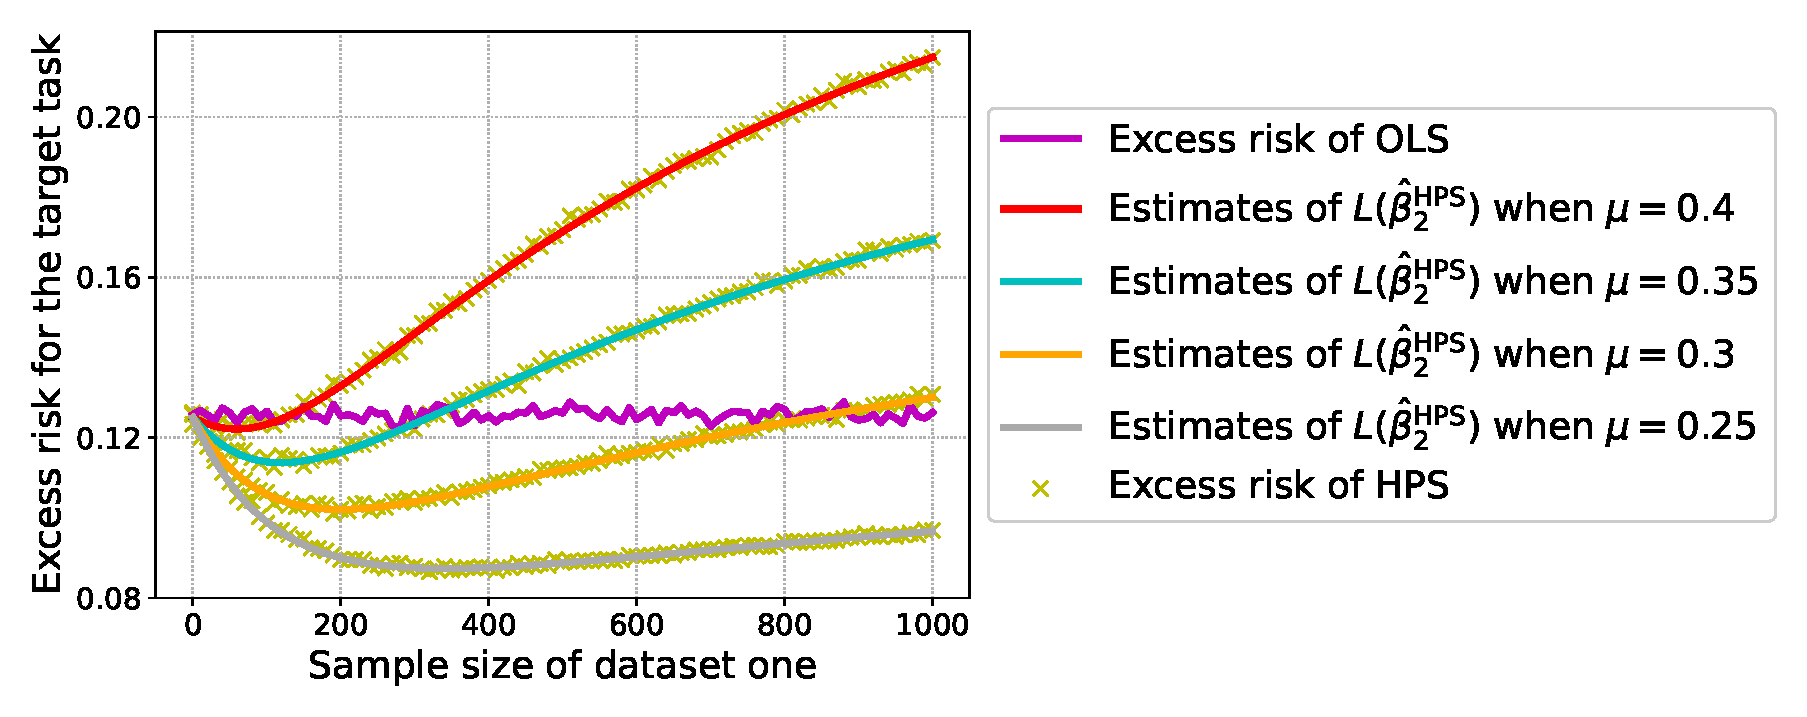
\includegraphics[width=0.8\textwidth]{figures/motivation.eps}
    \caption{We illustrate that our setup can reproduce the phenomenon of \textit{positive} (or \textit{negative}) \textit{information transfer}, which is prevalent in the context of transfer learning.
    We vary the sample size of dataset one and the distance parameter $\mu$ such that $\norm{\beta^{(1)} - \beta^{(2)}}^2 \approx 2\mu^2$. The region below the excess risk of the ordinary least squares (OLS) estimator corresponds to \textit{positive information transfer} when $L(\hat{\beta}_2^{\MTL})$ is smaller than the excess risk of the OLS estimator. This simulation uses $p = 100, n_2 = 300, \sigma = 1/2$. See also Figure \ref{fig_ab_data} for a similar phenomenon observed in text classification tasks.}
    \label{fig_motivation}
\end{figure*}

\subsection{Summary of results}

We consider a high-dimensional setting on each dataset where the sample size $n_i$ increases with $p$ to infinity proportionally by a constant factor, which has recently received lots of interests (see e.g., \citet{hastie2019surprises} and Section \ref{sec_related} for more references).
Let $\Sigma^{(i)} \in \real^{p\times p}$ be a deterministic positive semidefinite matrix.
The covariates are assumed to have population covariance equal to $\Sigma^{(i)}$:
\begin{align}
    x_j^{(i)} = \big(\Sigma^{(i)}\big)^{1/2} z_{j}^{(i)}, \text{ for any } j = 1,\dots,n_i, \label{eq_rvm}
\end{align}
where $z_j^{(i)}$ consists of independent and identical entries sampled from a distribution that has zero mean, unit variance, and satisfies certain bounded moment condition (see Section \ref{sec_data} for the precise assumptions).

We focus on the so called \textit{underparametrized} setting for the target task where $n_2 > p$ whereas for dataset one $n_1$ can be either smaller or greater than $p$.
Thus, the OLS estimator exists and it is well-known that the limit of its excess risk when $p$ approaches infinity is equal to $\frac{\sigma^2 p}{n_2 - p}$ (see e.g., \citet{bai2009spectral}).
By contrast, showing the asymptotic limit of $L(\hat{\beta}^{\MTL}_2)$ in the high-dimensional setting requires dealing with the inverse of the sum of two sample covariance matrices.
The first challenge is dealing with \textit{covariate shift}---when $\Sigma^{(1)}$ and $\Sigma^{(2)}$ are different.
The second challenge is dealing with \textit{model shift}---when $\beta^{(1)}$ and $\beta^{(2)}$ are different.
Our main result addresses both challenges by \todo{illustrate}.
\begin{itemize}
    \item \textbf{Covariate shift:}
    Our first result applies to settings where $\Sigma^{(1)}$ and $\Sigma^{(2)}$ can be arbitrarily different but $\beta^{(1)} = \beta^{(2)}$.
    For such settings, we show in Theorem \ref{thm_main_RMT} the asymptotic limit of $L(\hat{\beta}_2^{\MTL})$ as a function of the singular values of the matrix $\big(\Sigma^{(1)}\big)^{1/2}\big(\Sigma^{(2)}\big)^{-1/2}$ and the sample sizes $n_1, n_2$.
    \item \textbf{Model shift:} Our second result applies to settings where $\beta^{(1)}$ and $\beta^{(2)}$ can be arbitrarily different but $\Sigma^{(1)} = \Sigma^{(2)}$.
    For such settings, we show in Theorem \ref{cor_MTL_loss} the asymptotic limit of $L(\hat{\beta}_2^{\MTL})$ as a function of the $\ell_2$ distance between $\beta^{(1)}$ and $\beta^{(2)}$, and the sample sizes.
    \item \textbf{Covariate and model shift:} Our third result applies to settings with both covariate shift and model shift.
    When $\Sigma^{(2)}$ is isotropic, we show in Theorem \ref{???} the asymptotic limit of $L(\hat{\beta}_2^{\MTL})$ as a function of the singular values of $\Sigma^{(1)}$, the $\ell_2$ distance between $\beta^{(1)}$ and $\beta^{(2)}$), and the sample sizes.
    For the most general setting when $\Sigma^{(2)}$ is unisotropic, we show in Theorem \ref{prop_main_RMT} an estimate of $L(\hat{\beta}_2^{\MTL})$ that is accurate when $n_1$ is much larger than $n_2$.
\end{itemize}

Next, we demonstrate the power of these precise asymptotics by explaining a number of empirical phenomena in the context of transfer learning.
We consider a random-effect model where $\beta^{(i)}$ is equal to a shared model vector plus per-task variances (cf. \citet{dobriban2018high}).
Under this model, we show the following \textit{theoretical insights}.
\begin{enumerate}
    \item[i)] \textit{Whether or not covariate shift helps depends on sample sizes:} We consider the covariate shift setting and show that (cf. Proposition \ref{claim_dichotomy}) when $n_1 < n_2$, transferring from a data source with $\Sigma^{(1)} \neq \Sigma^{(2)}$ can achieve a smaller $L(\hat{\beta}_2^{\MTL})$ compared to transferring from a data source with $\Sigma^{(1)} = \Sigma^{(2)}$. When $n_1 > n_2$, transferring from from a data source with $\Sigma^{(1)} \neq \Sigma^{(2)}$ always results in higher $L(\hat{\beta}_2^{\MTL})$ than transferring from a data source with $\Sigma^{(1)} = \Sigma^{(2)}$.
    \item[ii)] \textit{Identical covariance provides approximately optimal transfer under imbalanced sizes:} Additionally, in Proposition \ref{prop_covariate}, we show that when $n_1$ is greater than $n_2$ times a certain large constant factor, transferring from a data source with $\Sigma^{(1)} = \Sigma^{(2)}$ achieves an approximately minimum excess risk value, within a certain family of covariance matrices of $\Sigma^{(1)}$.
    \item[iii)] \textit{Three regimes of information transfer under model shift}: Next, we consider the model shift setting and characterize the precise range of $n_1$ under which there is a positive transfer.
    In Proposition \ref{claim_model_shift}, we show that when $\mu^2 \le \frac{\sigma^2 p}{2(n_2 - p)}$ (recall that $\norm{\beta^{(1)} - \beta^{(2)}}^2 \approx 2\mu^2$) is small, the transfer effect is positive for any $n_1$.
    When $\frac{\sigma^2 p}{2(n_2 - p)} < \mu^2 < \frac{\sigma^2 n_2}{2(n_2 - p)}$, there is a transition from positive to negative transfer, as $n_1$ increases.
    When $\frac{\sigma^2 n_2}{2(n_2 - p)} \le \mu^2$, the transfer effect is negative for any $n_1$.
    Additionally, we illustrate that these three regimes of information transfer arises under both covariate and model shift (cf. Figure \ref{fig_sec3_cov_mo_b}).
\end{enumerate}

\paragraph{Empirical results.}
We also complement our theoretical analysis with empirical evaluations.
As mentioned in Section \ref{sec_mot}, our motivation for studying the HPS estimator stems from its superior empirical performance for transfer learning.
We affirm that HPS indeed outperforms several commonly used estimators including weighted averages of the OLS estimators of each task (cf. \citet{bastani2020predicting}) and the ridge estimator of the target task in our setting. See Figure \ref{fig_sec51} for the result.

We then conduct a case study on six text classification tasks using HPS neural network models.
We demonstrate that our theoretical insights above imply interesting new methods for mitigating covariate shift and model shift, respectively.

First, our insight ii) above suggests the importance of mitigating covariate shift under imbalanced dataset sizes.
To this end, we consider a certain covariance alignment procedure proposed in \citet{WZR20} for mitigating covariate shift.
We show that such an alignment procedure provides more significant improvement when $n_1 / n_2$ increases.

Second, our insight iii) above suggests subsampling the source dataset under model shift.
An efficient instantiation of this above would be to increase the sample size of the source dataset gradually until performance drops.
For example, in the setting of Figure \ref{fig_motivation}, this procedure will stop right at the minimum of the local basin.
On both two-task and multi-task case studies using the six text classification datasets, such a training procedure can reduce the computational cost by $65\%$ compared to a stochastic gradient descent procedure without sacrificing accuracy.


\paragraph{Extension to multiple sources.}
Finally, we also extend our setup to the case of having multiple data sources.
We consider a setting where all datasets have the same features but different labels, which is also known as multi-label prediction \cite{hsu2009multi}.
We show the asymptotic limit of $L(\hat{\beta}_i^{\MTL})$ under model shift (cf. Theorem \ref{thm_many_tasks}) and use the result to illustrate how to select the hidden width $r$ of $B$.
%Our result implies that when all tasks have the same features but different labels, for any task, HPS helps reduce the task's variance compared to single-task learning but increases bias.

%\medskip
%\noindent\textbf{Proof techniques.}
%There are two main ideas in our analysis. The proof of our first result uses a geometric intuition that hard parameter sharing finds a ``rank-$r$'' approximation of the datasets.
%We carefully keep track of the concentration error between the global minimizer of $f(A, B)$ and its population version (cf. equation \eqref{eq_A_star}).
%The proof of our second result is significantly more involved because of different sample sizes and covariate shifts. We show that the inverse of the sum of two sample covariance matrices with arbitrary covariate shifts converges to a deterministic diagonal matrix asymptotically (cf. Theorem \ref{thm_main_RMT}).
%We use recently developed techniques from random matrix theory to show a sharp convergence rate.
% to obtain a sharp estimate on the..., which is commonly referred to as the \emph{local law}.
%\HZ{add several sentences on the technical insight}
%One limitation of our analysis is that in Example \ref{ex_sample_ratio}, there is an error term that can result in vacuous bounds for very small $n_1$ (cf. equation \eqref{cor_MTL_error}).
%We believe our result has provided significant initial insights, and it is an interesting question to tighten our result.
%See Section \ref{sec_conclude} for more discussions of the technical challenge.



\subsection{Related work}\label{sec_related}


%Linear models in multi-task learning have been studied in various settings, including online learning \cite{CCG10,DCSP18}, sparse regression \cite{LPTV09,LPVT11}, and representation learning \cite{BHKL19}.

%Our setting is closely related to domain adaptation \cite{DM06,BB07,BC08,DH09,MMR09,CWB11,ZS13,NB17,ZD19}.
%The important distinction is that we focus on predicting the target task using a hard parameter sharing model.
%For such models, their output dimension plays an important role of regularization \cite{KD12}.
%Below, we describe several lines of work that are most related to this work.

%Some of the earliest works on multi-task learning are Baxter , Ben-David and Schuller \cite{BS03}.
%Mauer \cite{M06} studies generalization bounds for linear separation settings of MTL.
%The benefit of learning multi-task representations has been studied for learning certain half-spaces \cite{MPR16} and sparse regression \cite{LPTV09,LPVT11}.
%Our work is closely related to Wu et al. \cite{WZR20}.
%While Wu et al. provide generalization bounds to show that adding more labeled helps learn the target task more accurately, their techniques cannot be used to explain when MTL outperforms STL.
%\todo{spell out the challenge more explicitly}

%Ando and Zhang \cite{AZ05} introduces an alternating minimization framework for learning multiple tasks.
%Argyriou et al. \cite{AEP08} present a convex algorithm which learns common sparse representations across a pool of related tasks.
%Evgeniou et al. \cite{EMP05} develop a framework for multi-task learning in the context of kernel methods.
%\cite{KD12} observed that controlling the capacity can outperform the implicit capacity control of adding regularization over $B$.
%The multi-task learning model that we have focused on uses the idea of hard parameter sharing \cite{C93,KD12,R17}.
%We believe that our theoretical framework can apply to other approaches to multi-task learning.

\paragraph{Random matrix theory in machine learning.}
This work is inspired by an emerging line of recent work that has found random matrix theory useful for studying modern machine learning techniques.
A prominent line of recent work in this direction has been to understand the generalization properties of interpolators \cite{bartlett2020benign,hastie2019surprises,montanari2019generalization,liang2020just,liang2020precise}.
Interpolators such as minimum-norm estimators (in the context of linear regression) share similar behavior with modern neural networks in the sense that such models learn by ``memorizing'' the data with lots of parameters \cite{mei2019generalization}.
The study of such interpolators has also led to an explanation of the double-descent phenomenon \cite{belkin2019reconciling}.


\paragraph{Sample covariance matrices and distribution shift.}
These previous works primarily deal with a single high-dimensional sample covariance matrix. %need to check 
In the \textit{underparametrized} setting ($n_2 > p$) which this work focuses on, when the covariates are sampled from Gaussian distributions, the precise asymptotic limit can be derived directly from properties of the Wishart distribution (see also Lemma \ref{fact_tr} and the historical notes in Section \ref{sec_bv}).
In the high-dimensional setting, the eigenvalues of Wishart matrices satisfy the well-known Marchenko–Pastur (MP) law \cite{MP}, whose Stieltjes transform characterizes the variance limit.
Furthermore, it is well-known that the MP law holds universally regardless of the underlying data distribution of the covariates \cite{bai2010spectral}. \citet{isotropic} obtained a sharp convergence rate of the empirical spectral distribution (ESD) of the MP law for sample covariance matrices with isotropic population covariance matrices. \citet{Anisotropic,DY} later extended this result to sample covariance matrices with arbitrary population covariances. These results are proved by establishing certain optimal convergence estimates of the Stieltjes transforms of sample covariance matrices, which are referred to as \emph{local laws} in the random matrix theory literature. We refer the reader to \cite{erdos2017dynamical} and the references therein for a detailed review of related concepts.
Our technical contribution is to extend these techniques to the two-task setting and prove a local law for the sum of two sample covariance matrices with arbitrary covariate shifts.
Using the local law, we can then derive the variance limit with a precise dependence on the singular values of the covariate shift matrix $\big(\Sigma^{(1)}\big)^{1/2} \big(\Sigma^{(2)}\big)^{-1/2}$. 

%Our proof techniques use the so-called local law of random matrices, a recent development in the random matrix theory literature, called the \emph{local law} of 

%These techniques provide almost sharp convergence rates to the asymptotic limit compared to other methods such as free probability \cite{nica2006lectures}.
%We also extend the techniques in ?, which is one contribution of this work. 

%On the other hand, one may derive the asymptotic result in Theorem \ref{thm_main_RMT} with error $\oo(1)$ using the free addition of two independent random matrices in theory.

The asymptotic limit of the variance of $L(\hat{\beta}_2^{\MTL})$ (cf. equation \eqref{Lvar}) under covariate shift may also be derived using free addition in free probability theory \cite{nica2006lectures}.
However, this approach is not completely justified when the covariates are sampled from non-Gaussian distributions with non-diagonal covariate shift matrices. 
%(in the sense that it is hard to establish rigorously the free independence between two sample covariance matrices). 
Furthermore, our technique provides almost sharp convergence rates to the asymptotic limit, while it is unclear how to obtain such rates using free probability techniques, to the best of our knowledge.

The asymptotic limit of the bias of $L(\hat{\beta}_2^{\MTL})$ (cf. equation \eqref{Lbias}) involves ``asymmetric'' additions of two sample covariance matrices, whose analysis is technically involved.
Our result on the bias limit is inspired by the recent work of \citet{BES_free1,BES_free2}.
Additionally, we show a sharp convergence rate to the bias limit using free probability techniques.
Our work provides the first result in the model shift setting assuming that $\Sigma^{(1)} = \Sigma^{(2)}$ or that $\Sigma^{(2)}$ is isotropic, and the covariates are sampled from Gaussian distributions.
%To the best of our knowledge, we are not aware of any prior work on the precise bias limit in the high-dimensional setting, even for two Wishart matrices with the same population covariance matrix.
Showing the asymptotic bias limit under the most general covariate shift and model shift is an interesting open problem for future work.
See Section \ref{sec_conclude} for further discussion on the technical challenges.

\paragraph{Transfer learning and domain adaptation theory.}
Earlier works on transfer learning and domain adaptation use uniform convergence to obtain generalization bounds \cite{B00,BS03,M06}.
The influential paper by \citet{BBCK10} proposes a rigorous model for domain adaptation in classification (see also \citet{crammer2008learning} for an earlier result).
The main result provides a generalization bound for combining multiple data sources using an objective that averages over the risk of every datapoint.
This bound provides a principled way to reweight each data source by minimizing the bound.
From a technical perspective, uniform convergence based techniques provide upper bounds on the excess risks.
On the other hand, analyzing the empirical phenomena of information transfer such as the ones in Figure \ref{fig_motivation} requires tight lower bounds on the excess risks.

%One limitation of uniform convergence based techniques is that the results often assume that all  tasks have the same sample size, see e.g. \cite{B00,MPR16}.
%\citet{pontil2013excess}
%Moreover, these techniques do not apply to the high-dimensional setting because the results usually require a sample size of at least $p \log p$.
Finally, we discuss several concurrent works that study transfer learning in linear regression settings.
The work of \citet{li2020transfer} considers the problem of how to select useful data sources for transfer learning under model shift.
Their work provides an adaptive procedure that applies even when the set of useful data sources are unknown.
Our work differs from theirs in two aspects.
First, we considered a high-dimensional setting where the sample size increases with dimension proportionally.
Such a setting allows us to derive precise asymptotics of the excess risks, which is then used to explain a number of interesting phenomena in transfer learning.
Second, our result applies to covariate-shifted (and not necessarily Gaussian) source datasets whereas the setting of \citet{li2020transfer} assumes the covariates of all data sources and the target are drawn from a Gaussian distribution with the same population covariance matrix.
The work of \citet{lei2021nearoptimal} considers a setting of linear regression under distribution shift including covariate shift and model shift similar to our setting.
The difference is that our setting deals with a labeled target dataset whereas the result of \citet{lei2021nearoptimal} applies to settings with an unlabeled target dataset.
%One closely related work is \cite{WZR20}, which studied hard parameter sharing for two linear regression tasks.
%	\item \citet{kalan2020minimax}
%	\item \citet{lounici2011oracle}





\subsection{Organizations}
The rest of this paper is organized as follows.
In Section \ref{sec_HPS}, we formally define the data model and describe the underlying assumptions.
We show a bias-variance decomposition of the HPS estimator, and connect the bias and variance equations to random matrix theory.
In Section \ref{sec_main}, we show precise estimates for the excess risk of the HPS estimator under covariate and model shifts.
In Section \ref{sec_exp}, we evaluate the performance of HPS estimators against several commonly used transfer learning estimators, and present two implications for migating covariate and model shift in neural networks.
In Section \ref{sec_same}, we extend our setup to transferring from multiple data sources under model shift.
Section \ref{sec_conclude} concludes the paper and discusses potential future directions.
Section \ref{app_proof_error_same_cov}, \ref{appendix RMT}, and \ref{app_iso_cov} present proofs of our results.